\documentclass[aps,prd,reprint,amsmath,amssymb,superscriptaddress,nofootinbib,longbibliography,floatfix]{revtex4-2}
\usepackage[T1]{fontenc}
\usepackage{txfonts}
\usepackage{graphicx}
\usepackage{booktabs}
\usepackage{microtype}
\usepackage[hidelinks,pdfusetitle]{hyperref}
\graphicspath{{figures/}}

\begin{document}
\title{Central residence and density exposure of recoiling remnants in a Plummer potential}
\author{Venkata Hemanth Athota}
\email{bharadwaj.hemanth.002@gmail.com}
\affiliation{Independent researcher}

\begin{abstract}
We examine how accurately simplified central-residence prescriptions represent the density sampled by a recoiling remnant on an undamped orbit. For a test particle launched radially from the center of a static, isolated Plummer potential, we compute the first central-return time, finite-window central residence, and normalized density exposure using endpoint-regularized energy quadrature. Direct orbit integration and analytical limits provide independent checks. We compare continuous orbital exposure with uninterrupted central residence and with a prescription that suppresses exposure until first return, then assumes permanent central residence. The latter underestimates early exposure and eventually overestimates it because the undamped orbit repeatedly leaves the center. Near escape, the return time diverges while exposure per bound excursion approaches a finite limit. These results provide a reproducible collisionless benchmark for the stated prescriptions. They do not model frictional recentering or infer encounter rates, repeated-merger probabilities, or constraints from gravitational-wave observations.
\end{abstract}
\maketitle

\section{Introduction}\label{sec:introduction}
A retained merger remnant need not remain in the dense part of its host. Published work already studies recoil displacement and frictional recentering~\cite{Islam2026}, while hierarchical-merger calculations include host evolution and uncertain companion pairing~\cite{Torniamenti2024}. We isolate a narrower calculation: how accurately do assumed central residence and a first-return-then-central prescription reproduce the density sampled by an undamped orbit?

The experiment does not test the frictional-return model of Ref.~\cite{Islam2026}. Its first ballistic center crossing is distinct from dissipative recentering. Nor does it establish that an exact return time lacks orbital information: in this fixed one-parameter family, the return time and governing equations can identify the orbit. The subject is the error made by two explicitly defined approximations.

We use the standard Plummer potential~\cite{Plummer1911} as a smooth benchmark. The gravitational-wave connection is the post-recoil motion of a possible black-hole merger remnant; gravitational radiation, binary formation, and merger dynamics are not simulated here.

\section{Model and numerical method}\label{sec:model}
With host mass $M$, scale radius $b$, and gravitational constant $G$, define
\begin{align}
\Phi(r)&=-\frac{GM}{\sqrt{r^2+b^2}},\label{eq:potential}\\
t_d&=\sqrt{\frac{b^3}{GM}},\qquad
\eta=\frac{v_k}{\sqrt{2GM/b}}.\label{eq:units}
\end{align}
Let $x$ be signed displacement in units of $b$ and let time be measured in $t_d$. The initial-value problem is
\begin{align}
\ddot{x}&=-\frac{x}{(1+x^2)^{3/2}},\label{eq:motion}\\
x(0)&=0,\qquad \dot{x}(0)=\sqrt{2}\eta,\label{eq:initial}
\end{align}
with conserved dimensionless specific energy $E=\eta^2-1$.
We restrict attention to $0\leq\eta<1$. For a nonzero kick, $P$ is the interval between successive center crossings. Signed position has period $2P$; radius and density have period $P$. The exactly stationary case has no return event and is treated separately.

\subsection{First central return: experiment E001}\label{sec:return-method}
Energy conservation yields the apocenter
\begin{equation}
x_a=\frac{\eta\sqrt{2-\eta^2}}{1-\eta^2}\label{eq:apocenter}
\end{equation}
and return time
\begin{equation}
P=2\int_0^{x_a}\frac{dx}{\sqrt{2[(1+x^2)^{-1/2}-(1-\eta^2)]}}.\label{eq:period}
\end{equation}
Set $x=x_a\sin\theta$, $s=\sqrt{1+x_a^2\sin^2\theta}$, and $s_a=(1-\eta^2)^{-1}$. The endpoint singularity is removed:
\begin{align}
\frac{dt}{d\theta}&=\sqrt{\frac{s s_a(s+s_a)}{2}},\label{eq:transform}\\
P&=2\int_0^{\pi/2}\frac{dt}{d\theta}\,d\theta.\label{eq:regular-period}
\end{align}

\subsection{Residence and exposure: experiment E002}\label{sec:exposure-method}
For horizon $H$ and operational sphere radius $cb$, define
\begin{align}
C(H,c)&=\int_0^H\mathbf{1}_{|x(t)|<c}\,dt,\label{eq:residence}\\
I(H)&=\int_0^H(1+x(t)^2)^{-5/2}\,dt.\label{eq:exposure}
\end{align}
Here $C/H$ is a residence fraction, while $I/H$ is the mean host density relative to its central value. Neither is an encounter probability. The comparisons for nonzero kicks are
\begin{align}
I_{\mathrm{central}}(H)&=H,\label{eq:central}\\
I_{\mathrm{wait}}(H)&=\max(H-P,0);\label{eq:wait}
\end{align}
both equal $H$ for a stationary object.

The production calculation uses energy quadrature with absolute and relative tolerances of $10^{-11}$. Exposure integrals are split at radii 0.01, 0.1, 1, 10, and 100 when these lie on the orbit. This resolves narrow central passages at large apocenter. Complete periods accumulate exactly; the partial period is recovered by a bracketed inversion of outgoing travel time. Core crossing times are found by quadrature, not by a time-sampled indicator.

\section{First-return results}\label{sec:return-results}
E001 tabulates nine kick fractions from 0.1 to 0.999. The plotted curve extends to 0.9999. Table~\ref{tab:return} lists representative results, and Fig.~\ref{fig:return} compares the numerical curve with its asymptotic limits. All lengths and times use the units in Sec.~\ref{sec:model}.

\begin{table}[t]
\caption{Representative first-return results (E001). The apocenter is in units of $b$; $P$ is in units of $t_d$.}\label{tab:return}
% Generated from committed CSV results by paper/build.py.
\begin{ruledtabular}
\begin{tabular}{rrr}
$\eta$ & $x_a$ & $P$ \\
\hline
0.5 & 0.881917 & 4.395561 \\
0.8 & 2.591534 & 11.371439 \\
0.9 & 5.167285 & 27.972769 \\
0.95 & 10.207544 & 74.156668 \\
0.99 & 50.241305 & 792.551744 \\
0.999 & 500.249126 & 24856.344701 \\
\end{tabular}
\end{ruledtabular}

\end{table}

\begin{figure}[t]
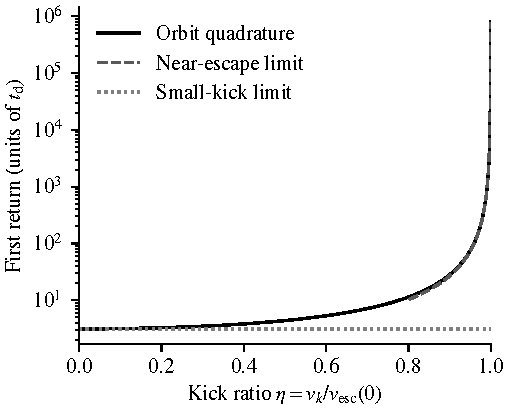
\includegraphics[width=\columnwidth]{return-time.pdf}
\caption{First central-return time from energy quadrature, with small-kick and near-escape limits. Binding alone does not imply a short excursion. The return is a crossing, not dissipative settling.}\label{fig:return}
\end{figure}

The small-amplitude equation is harmonic, so $P\to\pi$ as $\eta\to0^+$. At exactly zero kick, the particle instead remains stationary. Near escape,
\begin{equation}
P\sim\frac{\pi}{\sqrt{2}}(1-\eta^2)^{-3/2}.\label{eq:period-limit}
\end{equation}
At $\eta=0.99$, the apocenter is about $50b$ and the excursion takes about $793t_d$. Such large excursions also expose the limitations of the isolated potential: tides, external structure, or host evolution could materially alter a real remnant's trajectory. The tabulated values are conditional on the stated ideal model.

\section{Residence and exposure results}\label{sec:exposure-results}
E002 uses 11 kicks from 0 to 0.999 and spheres with $c=0.1,0.3,1$. Seven fixed horizons span 1 to 1000 dynamical times. For the ten nonstationary kicks, a second grid uses $H/P=0.1,0.5,1,2,10$. Fixed and period-scaled windows are distinct comparisons.

\begin{table}[t]
\caption{Density exposure and residence over one radial period (E002). All entries are dimensionless; $C(P,1)/P$ is the fraction of a period inside $r<b$.}\label{tab:exposure}
% Generated from committed results by paper/build.py.
\begin{ruledtabular}
\begin{tabular}{rrrr}
$\eta$ & $I(P)$ & $I(P)/P$ & $C(P,1)/P$ \\
\hline
0.3 & 2.774830 & 0.793277 & 1 \\
0.8 & 1.369228 & 0.120409 & 0.174465 \\
0.99 & 1.029215 & 0.00129861 & 0.0019312 \\
\end{tabular}
\end{ruledtabular}

\end{table}

At $\eta=0.99$, the time inside $r<b$ is 1.530574 dynamical times per radial period. The mean sampled density is approximately $0.130\%$ of the central value, while the residence fraction inside this sphere is $0.193\%$ (Table~\ref{tab:exposure}). These percentages describe one ideal orbit, not an observed population.

\begin{figure*}[t]
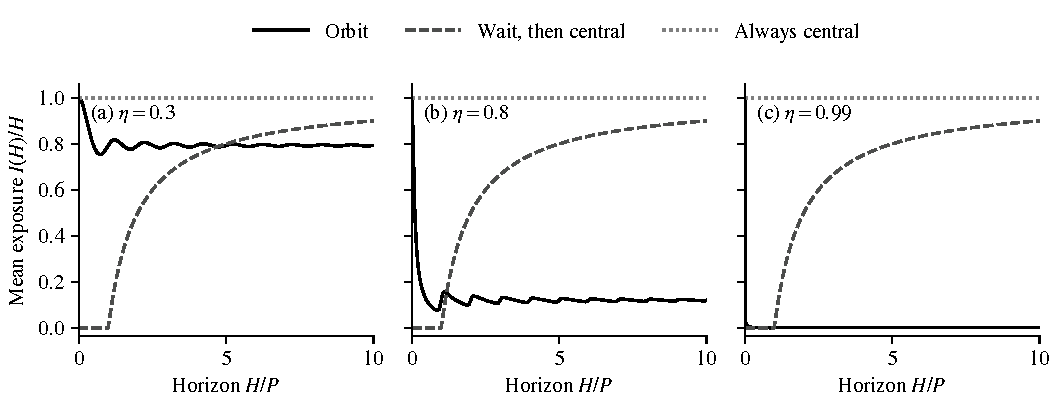
\includegraphics[width=\textwidth]{exposure-comparison.pdf}
\caption{Mean normalized density sampled up to each horizon for three kick fractions: (a) $\eta=0.3$, (b) $\eta=0.8$, and (c) $\eta=0.99$. The first-return comparator suppresses all initial exposure and then assumes unit density permanently. The undamped orbit repeatedly departs from the center. Line styles distinguish the prescriptions independently of color.}\label{fig:exposure}
\end{figure*}

At $H=P$, the wait prescription gives zero, whereas the orbit has accumulated $I(P)>0$. At $H=10P$ for $\eta=0.99$, the orbit gives 10.292151 dynamical times of exposure and the wait prescription gives 7132.965700. The error changes sign (Fig.~\ref{fig:exposure}). More generally, as $H$ grows, the wait prescription approaches unit mean density while the orbit approaches $I(P)/P<1$ for every nonzero kick. It is therefore not uniformly conservative.

An orbit stays within a sphere when its apocenter does not exceed its radius:
\begin{equation}
\eta\leq\sqrt{1-\frac{1}{\sqrt{1+c^2}}}.\label{eq:threshold}
\end{equation}
For $c=1$, the threshold is 0.541196. Equality touches the sphere boundary instantaneously and does not change an integrated residence fraction. Even an orbit entirely within the sphere samples a varying density; residence and density exposure are different quantities. Figure~\ref{fig:residence} shows the dependence on the operational sphere radius.

\begin{figure}[t]
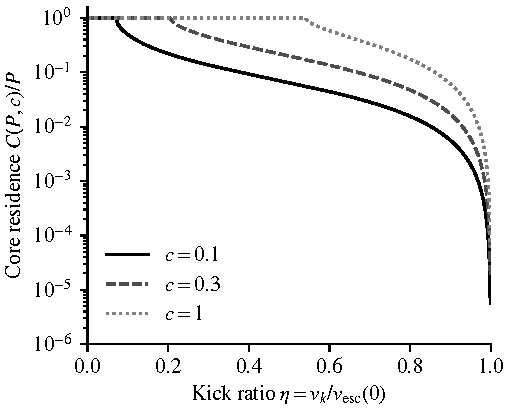
\includegraphics[width=\columnwidth]{core-residence.pdf}
\caption{Residence fraction per radial period for three operational sphere radii. Each curve equals unity below the threshold in Eq.~\eqref{eq:threshold} and decreases as bound kicks approach escape. The radii are model definitions, not measured cluster core radii.}\label{fig:residence}
\end{figure}

\section{Analytical and numerical verification}\label{sec:validation}
For a stationary object, $I(H)=C(H,c)=H$. For nonzero bound kicks, both exposure and occupancy repeat every $P$, hence $I(nP)=nI(P)$. In the small-kick limit, $I(P)\to\pi$ and $I(P)/P\to1$.

Near escape, the marginally bound outgoing trajectory obeys $\dot{x}=\sqrt{2}(1+x^2)^{-1/4}$. The limiting exposure of a full bound excursion is
\begin{align}
\lim_{\eta\to1^-}I(P)
&=\sqrt{2}\int_0^\infty(1+x^2)^{-9/4}dx\notag\\
&=\sqrt{\frac{\pi}{2}}\frac{\Gamma(7/4)}{\Gamma(9/4)}\notag\\
&\simeq1.0166557018.\label{eq:exposure-limit}
\end{align}
Combining this with Eq.~\eqref{eq:period-limit} gives
\begin{equation}
\frac{I(P)}{P}\sim\frac{\Gamma(7/4)}{\sqrt{\pi}\Gamma(9/4)}(1-\eta^2)^{3/2}.\label{eq:mean-limit}
\end{equation}
This is a limit from bound orbits. An exactly marginally bound particle does not return in finite time.

The recorded verification contains 27 passing tests. Independent checks integrate the signed equations of motion using DOP853~\cite{SciPySolveIVP}, compare central crossings, monitor energy, and integrate accumulated density as an additional state variable. Core residence is checked with event-segmented trajectories. Other tests cover stationary behavior, sphere thresholds, period accumulation, crossing continuity, density as the derivative of exposure, invalid inputs, and convergence near escape. The strongest near-escape numerical cases reach $\eta=0.9999$; no claim is made of uniform numerical accuracy arbitrarily close to escape.

Separately, the result verifier reproduces 146 recorded rows: nine return-time rows, ten cycle rows, 77 fixed-window rows, and 50 period-scaled rows. It also checks the recorded input and output hashes. This second step verifies stored results against their implementation; it is not an additional independent physics calculation. Numerical tolerances are solver controls, not error bars on the physical model.

\section{Discussion and conclusions}\label{sec:conclusions}
The two tested prescriptions fail to preserve continuous exposure for distinct reasons: one assumes uninterrupted central residence, and the other removes the initial outbound passage before imposing permanent central residence. The first-return-then-central prescription misses early exposure and eventually overestimates late exposure. Exposure per bound excursion remains finite as the return time diverges toward escape.

Density exposure does not supply a companion distribution, relative-velocity distribution, encounter cross section, binary fraction, or companion-acquisition mechanism. The potential is static and isolated, and the test particle does not experience friction, scattering, or tidal removal. Consequently, these results do not estimate a repeated-merger probability, distinguish astrophysical formation channels, or replace evolving cluster calculations~\cite{Torniamenti2024}. The results quantify the two prescriptions within a controlled orbital benchmark.

\section*{Data and code availability}
The implementation, configurations, generated tables, verification code, figures, and manuscript source are available in the version 0.1.1 research release~\cite{AthotaSoftware}. Python 3.11 is the numerical reference environment; dependencies are pinned. The experiment manifest records the generating source commit, source and output hashes, and runtime versions. The paper manifest separately records its build inputs and outputs. Project-authored code and documentation are distributed under the MIT license. No observational data are used.

\bibliography{references}
\end{document}
